\documentclass[12pt,a4paper,titlepage]{report}

% Document Info
%
\newcommand\AcademicTitle{Dynamic Performance Framework}
\newcommand\CommericalTitle{Iris}
\newcommand\Author{Dean Gaffney}
\newcommand\StudentID{20067423}
\newcommand\Date{December 2017}
\newcommand\Report{Status Report (Semester 2)}
\newcommand\Reader{Supervisor: Dr.~Kieran Murphy}
\newcommand\SecondReader{Second Reader: David Drohan}

\usepackage{fyp_document}

\newcommand*{\mybox}[2]{\colorbox{#1!30}{\parbox{.98\linewidth}{#2}}}
\newcommand{\q}[1]{``#1''}

\begin{document}

\pagenumbering{roman}

% title page as per Ian's spec
\thispagestyle{empty}
\begin{center}
\mbox{}\vfill
{\fontsize{18pt}{20pt}\selectfont \bfseries \AcademicTitle}
\vfill
{\fontsize{14pt}{20pt}\selectfont \bfseries\itshape \CommericalTitle}
\vfill
{\fontsize{12pt}{20pt}\selectfont \bfseries \Report}
\vfill
{\fontsize{14pt}{20pt}\selectfont \bfseries \Author}
\vfill
{\fontsize{14pt}{20pt}\selectfont \bfseries \StudentID\ Panel 3}
\vfill
{\fontsize{14pt}{20pt}\selectfont \bfseries \Reader}
\vfill
{\fontsize{14pt}{20pt}\selectfont \bfseries \SecondReader}
\vfill
{\fontsize{14pt}{20pt}\selectfont \bfseries BSc (Hons) in Entertainment Systems}
\vfill
\end{center}
\clearpage

\tableofcontents
\listoftables
\listoffigures

% start of main matter
\clearpage
\pagenumbering{arabic}
\setcounter{page}{1}

\chapter{Abstract}

The aim of this project is the design a full implementation of a system for application performance monitoring. The proposed system, has the working title,  Iris.

On completion, Iris will provide users with a dynamic performance framework which will allow users to fully customise and centralise their application performance monitoring. This will be achieved through a web interface where a user can specify a schema for a specific application they wish to monitor. Once a schema has been set up, a REST endpoint will be generated for the application. This endpoint will allow a user to send their monitoring data from their desired application to the framework in the form of JSON (matching the specified schema). Iris will also contain features which allow a user to monitor and analyse incoming data, using an intelligent, fully customisable graph and dashboard builder. Iris will then visualise any received data in real time using to the appropriate dashboards using websockets. Iris will come with some out of the box scripts/applications that users can use to monitor typical tasks such as JVM (Java Virtual Machine) performance, Linux OS System Performance.

\chapter{Introduction}

\section{Motivation for Iris}

The motivation for this project comes from database and system performance issues that Onaware\footnote{Onaware is an international company that specialises in IAM (Identity and Access Management) and has offices with 20 staff in Waterford. More information on Onaware can be found at \url{https://onaware.com}.} has experienced in recent projects. It is often the case that they must deal with large amounts of identity data being aggregated into a third party system called `IIQ'.

Onaware has faced major issues with aggregating data in the past, in some cases it was taking up to five days, and sometimes they would fail halfway through meaning aggregations would have to be restarted, due to the amount of software involved it is hard to pinpoint what software is causing the issue.

In one such instance of aggregating data issues several attempts were made to rectify the performance issue such as optimising sql queries, increasing ram, multi threading tasks and increasing disk space, none of which worked. Due to the performance issue the IIQ instance became unusable so debugging the issue was not possible from inside the application and log files became so big that text editors would crash when trying to open them. In this case the issue turned out to be a customer putting size constraints on the database storing the aggregated data. While monitoring would not prevent such a mistake it would have reduced the time needed to locate the issue.

In response to difficulties in identifying performance issues Onaware have tried to monitor specific application elements. The aim at the time was to try and combine SQL, JVM and Operating System scripts to track the performance of the tools, however this approach is not very scalable and it would need to be reconfigured for future projects.

Iris is an attempt to solve this problem. Iris will allow a user create a new application monitor with little effort using a web interface, give the user a REST endpoint specific to the application for their scripts to target their data, and allow a user to monitor the data in real time using graphs and dashboards. The aim is to make the framework as flexible as possible and not specific to the issue Onaware faced, meaning a user can monitor any data they want from any application they want all they must do is send their data to a REST endpoint.

Users of Iris will consist of Onaware developers who will be monitoring IAM project data and generic tools which may be released to clients at a later time.

\section{Features List}
\subsection{Types of data}
numerical, categorical and textural

\chapter{Implementation}
During semester 1 a number of implementation were designed and tested. As a result the implementation described in
semester 1 required not further changes in thus sesmter,. Hence, this section is fundamentally unchanged from that in
semester 1 report
Distinguish between subparts that were implemented (and so their overview here is similar to that in semester 1 report) and
subparts that were implemented during this semester (and so the overview here is new).
In this chapter the implementation of Iris is summarised. The components completed in semester were described in the
Semester 1 report and that summary is reproduced here (with minor modification) for completeness. The subsections dealing
with components impleneted in semester 2 is fundmental new. Table REF lists the components adn when they were completed.
\begin{center}
\begin{tabular}{llll}
Component                         & When prototyped  & When completed \\\hline
code framework/services  & Semester 1 & Semester 1 \\
schemas &\\
dashboards &\\
aggregiation builder  &\\
data sources & \\
\end{tabular}
\end{center}

\section{Core Framework/Services}
\section{Schemas}
\section{Dashboards}
\section{Aggregation Builder}
\section{Data Sources}

\chapter{Deployment, Testing and Evaluation}

\section{Deployment}
\subsection{AWS}
\subsection{Jetty}
\subsection{Gradle}
\subsection{WAR}
\subsection{MySql GORM Mapper}

\section{Testing and Evaluation - Data Sources}
\subsection{Introduction}
A number of data source have been implemented to demonstrate the flexibility of Iris and to test the aggregation. Each
of the following sections describe a data source and its unique features.

\subsection{Android App}
\subsubsection{Description}
The android application demonstrates how Iris handles state based data. The application is very simple, but demonstrates how simple it is to monitor an application's state through Iris. The application is simply a screen consisting of six tiles. Each tile represents a different state, each state has three colours and three numerical values linked to the states and colours. The android application allows the user to change the states of these tiles, which then changes the state of the tile colour and value. When a user is satisfied with the states they wish to send to Iris they simply tap the screen. This results in a JSON object being sent to Iris consisting of the current numerical value for each state tile i.e the current state of the tiles.
%Iris Android app screenshot
\begin{figure}[H]
\begin{tcolorbox}
\begin{center}
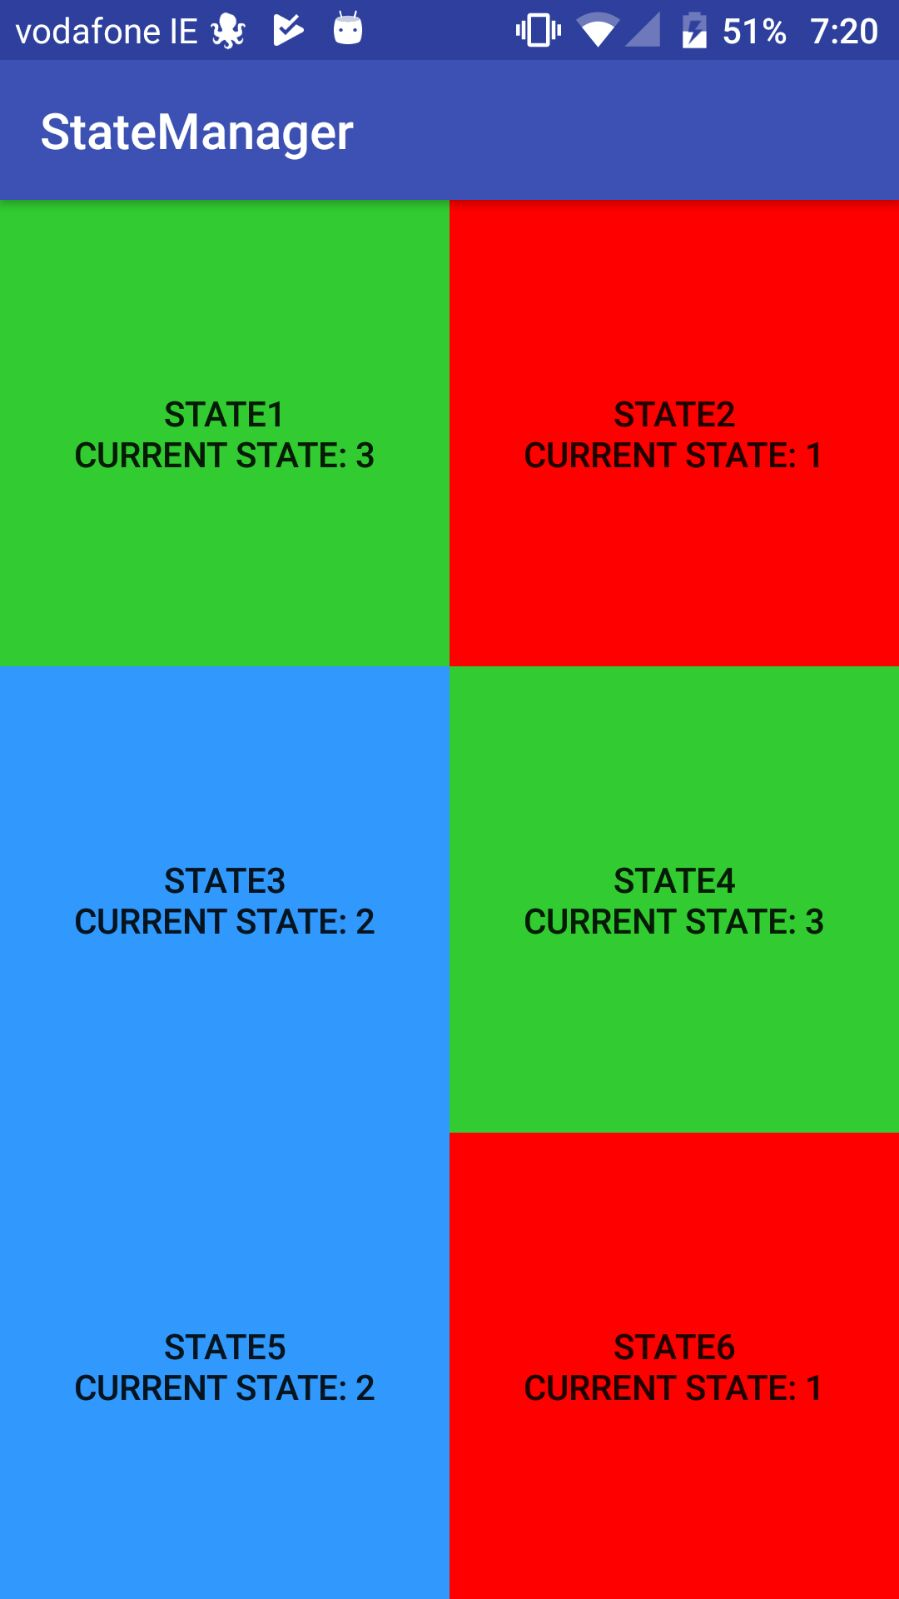
\includegraphics[width=0.7\textwidth,height=0.7\textheight]{android-agent}
\end{center}
A screenshot of the android agent and its state based tiles.
\end{tcolorbox}
\caption{Android agent for Iris}
\end{figure}

\subsubsection{Linkage with Iris}
The android application is linked to Iris through a unique REST endpoint specific to the android application. All of the data being sent from the android application is sent to this endpoint. Once the data enters Iris, Iris will run through it's logic for checking for dashboards and charts associated with the schema and send the data through to the charts. 
%Add a ref to a section where you explain what iris does, so you dont have to keep repeating this for all agents
In this case the charts are state based and will update according to the state values that are given to them.
%Iris Android agent dashboard screenshot
\begin{figure}[H]
\begin{tcolorbox}
\begin{center}
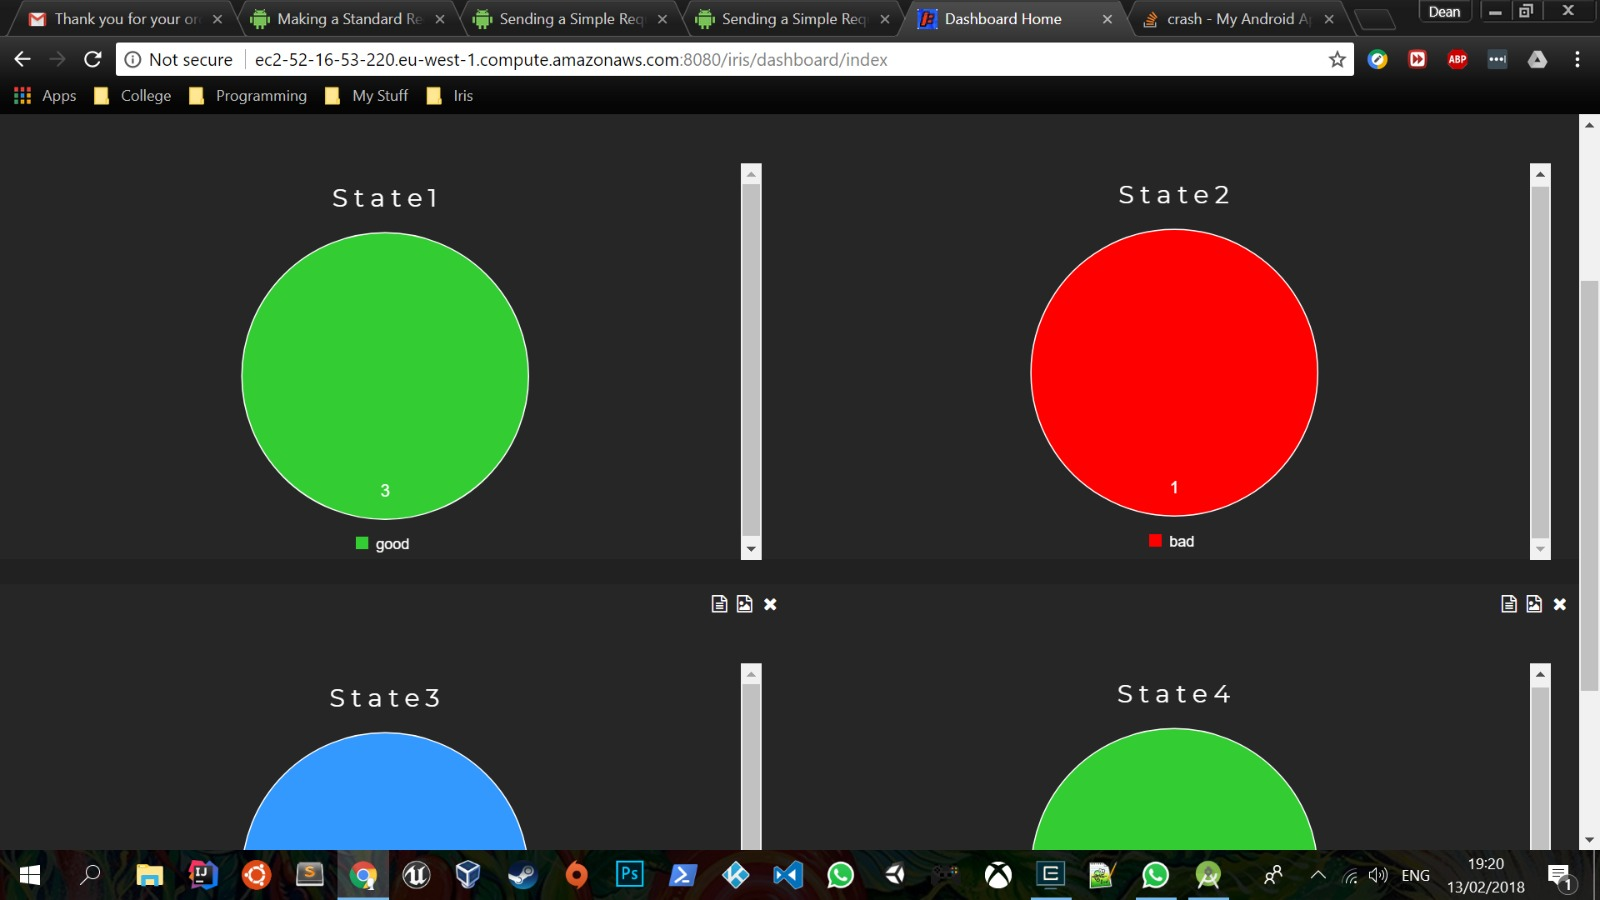
\includegraphics[width=\textwidth,height=\textheight,keepaspectratio]{iris-android-dashboard}
\end{center}
A screenshot of the android agent dashboard in Iris and its state based tiles.
\end{tcolorbox}
\caption{Android agent dashboard in Iris}
\end{figure}


\subsection{Raspberry Pi}

%Crypto-currency script
\begin{figure}[H]
\begin{tcolorbox}
\begin{minted}{python}

\end{minted}
\end{tcolorbox}
\caption{iris-crypto-rates.py soure code}
\end{figure}

\subsubsection{Description}
What's so special about this data source?
\subsubsection{Linkage with Iris}
Resulting dashboard (some images)

\subsection{Nodejs}
\subsubsection{Description}
What's so special about this data source?
\subsubsection{Linkage with Iris}
Resulting dashboard (some images)

\subsection{Selenium}
\subsubsection{Description}
What's so special about this data source?
\subsubsection{Linkage with Iris}
Resulting dashboard (some images)

\subsection{MySQL}
\subsubsection{Description}
What's so special about this data source?
\subsubsection{Linkage with Iris}
Resulting dashboard (some images)

\chapter{Conclusions}



\nocite{*}
\printbibliography

%%%%%%%%%%%%%%%%%%%%%%%%%%%%%%%%
\clearpage

\begin{appendices}

\end{appendices}
\end{document}
